% Document template based on LNCS, adapted by Matt Welsh <mdw@cs.berkeley.edu>

% This version is adapted to use PDFTEX to render to PDF directly. 
% If you want to use dvi, you need to change any figures to use '.eps'
% rather than '.pdf', and probably get rid of the hyperref package.

%\documentclass[11pt, onecolumn, draftcls]{IEEEtran}
\documentclass[11pt]{IEEEtran}
\usepackage{program}
\usepackage{epsfig}
\usepackage{url}
\usepackage[english]{babel} % mdw: Required to get good hyphenation on RH6.0
                            % (fixed in RH6.1)
\usepackage{graphicx} 
\usepackage{color}    
\usepackage{cite}

\newcommand{\XXXnote}[1]{{\textcolor{red}{\bf MDW: #1}}}
\newcommand{\GWAnote}[1]{{\textcolor{red}{\bf GWA: #1}}}
%\newcommand{\XXXnote}[1]{}
%\newcommand{\GWAnote}[1]{}

\pagestyle{empty}
\begin{document}

%don't want date printed
\date{}

%%%%%%%%%%%% THIS IS WHERE WE PUT IN THE TITLE AND AUTHORS %%%%%%%%%%%%


% MDW: We need to say "Wireless Sensor Network" here
%\title{Developing a Wireless Sensor Network for High-Bandwidth, High-Fidelity
%Volcanic Monitoring}

\title{Deploying a Wireless Sensor Network on an Active Volcano}
\def\footnotemark{}

\author{\authorblockN{Geoffrey Werner-Allen\authorrefmark{1}, 
Konrad Lorincz\authorrefmark{1}, 
Mario Ruiz\authorrefmark{2}\authorrefmark{4}, 
Omar Marcillo\authorrefmark{3}\authorrefmark{4}, 
Jeff Johnson\authorrefmark{2},
Jonathan Lees\authorrefmark{3},
and Matt Welsh\authorrefmark{1}} \\
\authorblockA{\authorrefmark{1} Division of Engineering and Applied
Sciences, Harvard University} \\
\authorblockA{\authorrefmark{2} Dept. of Earth Sciences, University of
New Hampshire} \\
\authorblockA{\authorrefmark{3} Dept. of Geological Sciences, University of 
North Carolina} \\
\authorblockA{\authorrefmark{4} Instituto Geof\'{i}sico, Escuela 
Polit\'{e}cnica Nacional, Ecuador}}

%\author{\authorblockN{Geoffrey Werner-Allen, Konrad Lorincz, and Matt
%Welsh\\}
%\authorblockA{Harvard University, \{werner,konrad,mdw\}@eecs.harvard.edu\\}
%\authorblockN{Mario Ruiz and Jonathan Lees\\}
%\authorblockA{University of North Carolina, \{mruiz,leesj\}@email.unc.edu\\}
%\authorblockN{Omar Marcillo and Jeff Johnson\\}
%\authorblockA{University of New Hampshire,
%\{omar.marcillo,jeff.johnson\}@unh.edu}
%}

\maketitle
\thispagestyle{empty}

%%%%%%%%%%%%%  ABSTRACT GOES HERE %%%%%%%%%%%%%%

\begin{abstract} 
Wireless sensor networks have the potential to aid the study of active
volcanoes.  Augmenting heavy and power-hungry data collection
equipment with lighter, smaller wireless sensor network nodes leads to
faster, larger deployments.  Arrays consisting of dozens of wireless sensor
nodes are now possible.  The additional scale and resolution of these
networks permits scientific studies not feasible with traditional
instrumentation.  Designing sensor networks to support volcanic studies
requires addressing the high data rates and high data fidelity these studies
demand.  We have designed a sensor network application for volcanic data
collection that relies on triggered event detection and reliable data
retrieval to meet bandwidth and data quality demands.  Here we describe our
design and relate our experience deploying our network on Volc\'{a}n
Reventador, an active volcano in northern Ecuador.  
\end{abstract}

\chapter{Introduction}
\label{chap-intro}

An emerging application for wireless sensor networks is their use in medical
care. Many medical applications place new demands on sensor network designs.
They often involve variable data rates, multiple receivers, and mobile
nodes. Most existing sensor network designs do not adequately support these
requirements, focusing instead on aggregating small amounts of data from nodes
at fixed locations. Therefore a gap exists between existing sensor network
architectures and the requirements of medical applications.

In this dissertation, we bridge the gap by making three contributions: we
propose CodeBlue medical sensor network architecture, TinyADMR ad-hoc multicast routing protocol, and LiveNet passive monitoring infrastructure.
With CodeBlue, we address the challenges of providing a flexible 
and implementable system architecture for mote-based medical
sensor networks. TinyADMR addresses challenges in multicast routing with the
existence of low quality radio links, memory and bandwidth limitations.
LiveNet addresses the challenges for evaluating deployed medical sensor
networks by reconstructing network dynamics without introducing additional
overhead to the network. We evaluate CodeBlue, TinyADMR and LiveNet
with an indoor sensor network testbed and with a disaster drill deployment.

\section{Medical sensor networks}

The convergence of several new hardware technologies, including MEMS, low
power processors, and low power radio, has enabled a new class of computing
platform: wireless sensors. Wireless sensors combine the capability of
sensing, computation, and wireless communication into a single physical
package, enabling a wide range of applications. Over the past decade, sensor
networks research community has explored the use of wireless sensors in
military target tracking and environmental monitoring such as habitats,
forests, volcanoes, civil infrastructures, factory equipments, and home energy
usage.

One common characteristic of most conventional sensor networks is that they
are intended for deployments of stationary nodes that transmit data at
relatively low rates, with a focus on best-effort data collection at a central
base station. Although the sensor networks research community has made
tremendous progress in perfecting networking and operating system support in
this space, we argue that there is a lack of adequate architectural
support for one emerging and important application domain: medical care.

In a hospital or clinic, outfitting every patient with tiny,
wearable wireless vital sign sensors allows doctors, nurses and other
caregivers to continuously monitor the status of their patients.  In
an emergency or disaster scenario, the same technology would enable
medics to more effectively care for large numbers of casualties.
First responders could receive immediate notifications on any changes
in patient status, such as respiratory failure or cardiac arrest.
Wireless sensors can augment or replace existing wired telemetry
systems for many specific clinical applications, such as physical
rehabilitation or long-term ambulatory monitoring.

A typical scenario involves many patients wearing sensors that monitor basic
vital signs such as heart rate or blood oxygen saturation. A small number of
medical personnel are responsible for continuously monitoring the patients
using devices such as laptops or PDAs. Using the real-time information
retrieved from the network, the medical team can treat
patients who need urgent care more efficiently.


\subsection{Application requirements}

Medical sensor networks have several different characteristics than
conventional sensor network applications. The sensors are worn by patients and the
data sinks are mobile computers carried by doctors or nurses so that the nodes
in the network are not stationary. Unlike typical sensor networks, there are
likely to be more than one data sinks in the network. Nodes can also join or
leave the network dynamically. Furthermore, the data traffic pattern is
on-demand and dynamic. Different doctors may be interested in real-time status
of different groups of patients and the groups can potentially overlap. There may
also be interests for different types or resolutions of sensor data.
Conventional sensor network architectures are inadequate in such scenarios
because the system cannot assume fixed sensor queries, sampling rate and
static traffic pattern. 


%% data may have different priorities associated with it

\subsection{Resource limitation}

In addition to meeting a different set of application requirements, medical sensor
networks, as conventional sensor network systems, face the challenges from
severe
resource limitations of the low power sensor platforms. To be practical, the
sensor nodes must be light-weight, low power and low cost so that they can be
wearable, have long enough battery lifetime and be affordable. This entails
the use of low power radio and low power processor.  For example, the mote
platform, MicaZ~\cite{micaz}, that we use for our medical sensor networks has
4~KB of RAM, a 4~MHz 8-bit CPU and a low power IEEE 802.15.4 radio with
maximum transmit power at 0 dBm. The implication of such a limited platform is
that the software running on the mote cannot be overly computationally
intensive or require large amount of memory. Yet, the system must be responsive enough
to handle complex
interactions with the environment such as sampling medical sensors and
performing radio communication in time. As a result, we not only have to find
a new architecture that fulfills the application requirements, it must also be
designed carefully so that it is light weight enough to fit into the platform
but complex enough to fulfill the application demands. 

\section{Systems challenges for medical sensor networks}

We outline a set of challenges identified through the process of designing,
implementing, deploying, and evaluating a medical sensor network. First of
all, there needs to be a new network architecture to efficiently support the
type of queries and traffic patterns for medical sensor networks. Secondly,
to support the new architecture, it is necessary to provide multicast routing
capability on resource-limited sensor nodes. Third, studying a deployed
medical sensor network requires a non-trivial network monitoring infrastructure.

\subsection{A new network architecture}

In contrast to conventional sensor network applications, medical monitoring
must support a large number of patient sensors deployed in a hospital or
disaster site, a variety of data rates, and multiple mobile receiving
devices, such as PDAs carried by doctors or medics. Moreover, medical
monitoring cannot make use of traditional
in-network aggregation since it is not generally meaningful to combine data
from multiple patients. The goal is instead to efficiently deliver information
to the correct receivers. Therefore, there is a significant gap between
existing sensor network designs and the requirements of medical monitoring. 

Supporting such broad range of requirements demands a new approach to
sensor network design. To bridge the technology gap, we propose CodeBlue, an
architecture for medical sensor networks that provides a set of protocols and
services tailored for this application domain. CodeBlue includes
a publish/subscribe communication model, a rich query interface for periodic
and triggered collection of sensor data, a dynamic sensor discovery protocol,
and a programmatic external interface based on Web Services standards.
CodeBlue provides a high-level interface to the network, making it easy to
support new sensor types and applications that tie into real-time medical
sensor data.

\subsection{Multicast on resource limited sensor nodes}

By reviewing the application requirements of medical sensor networks, it
becomes clear that an ad-hoc multicast routing protocol is more adequate
than the conventional many-to-one data collection tree routing approach.
Fortunately there are existing multicast protocols designed for ad-hoc mobile
networks. However, after the attempt to implement one such protocol, ADMR, on
our resource limited sensor platform, we have discovered several challenges
that were not foreseen by the original designers. In order to achieve
acceptable packet delivery ratio, we have to use different routing metrics that
involves the use of link quality information. We have also
investigated the challenges to scale the network within the memory and
bandwidth limitations on the sensor platform.

\subsection{Deployment support}

To find out whether a design is practical for realistic use, one needs to
deploy the network and evaluate the performance in a realistic environment.
For this purpose, we have conducted a deployment study of the CodeBlue
network. It is necessary to record system behavior in order to study
the correctness and performance of the network during the deployment. Under severe
resource constraints on CPU, memory and bandwidth, it is not practical to
record such information on the sensor nodes locally or transmit the logged
information over the radio. To overcome this problem, we have designed and
built LiveNet, an entirely passive monitoring infrastructure for
reconstructing dynamics of deployed sensor networks.  LiveNet is passive and
therefore does not require changing the application code or incur any
additional resource consumption in the network. Yet, it is able provide
valuable information for evaluating and debugging the deployed network.

\section{Dissertation outline}

The remainder of the dissertation is organized as follows.

Chapter 2 considers background and related work. This chapter introduces 
existing work in sensor networks and ad-hoc networking research community that 
are related to medical sensor networks. We also provide an overview of target
hardware platforms of this thesis.

Chapter 3 presents the requirements for a large class of medical sensor
network applications and a new software architecture to meet these
needs. We first propose the CodeBlue network architecture by presenting the
system goals and overall architecture design. We then describe individual
components
to discuss the design trade-offs in detail. Our key contributions include
proposing publish/subscribe as the appropriate networking abstraction for
a medical sensor network and designing CodeBlue Query (CBQ) interface, which
provides a programmatic interface to the medical sensor network.

Chapter 4 presents our approach to achieving efficient publish/subscribe
communication in sensor networks with mobile nodes, based on the
ADMR~\cite{admr-mobihoc01} {\em ad-hoc\/} multicast routing
protocol. We first describe the challenges encountered when designing and 
implementing the multicast layer to support publish/subscribe communication 
model for CodeBlue. We identify the
challenges from unreliable wireless radio links, memory constraints and
bandwidth constraints. We also explore and evaluate different route discovery
and expiration strategies. The key contributions include two new 
routing metrics that exploit link quality information and identifying
scalability limitations from memory and bandwidth constraints.

Chapter 5 describes LiveNet passive monitoring infrastructure. This chapter 
covers the architecture of LiveNet that involves passive sniffers, trace
merging algorithm and a set of analyses that are used to analyze CodeBlue
deployments. We also present the results of an extensive validation study of 
LiveNet's performance and accuracy with a set of controlled experiments with 
an indoor testbed, MoteLab.

Chapter 6 covers implementation and detailed performance evaluation of
CodeBlue network architecture.  We present evaluation of CodeBlue both on a
sensor network testbed and with a disaster drill deployment.  The testbed
experiments evaluate CodeBlue in scalability, fairness, latency, jitter and
effect of mobility. Then we present a deployment study that was part of a disaster
drill simulating a bus accident. Using data from LiveNet, we are able to
analyze the traffic load, network hotspots, routing paths, and query yield for
this deployment.

Chapter 7 contains lessons learned from the experience of 
designing, implementing, deploying and evaluating medical sensor networks and
provide potential future research directions. 

Chapter 8 concludes.

\section{Overview of Three Deployments}

\begin{figure}[t]
\begin{center}
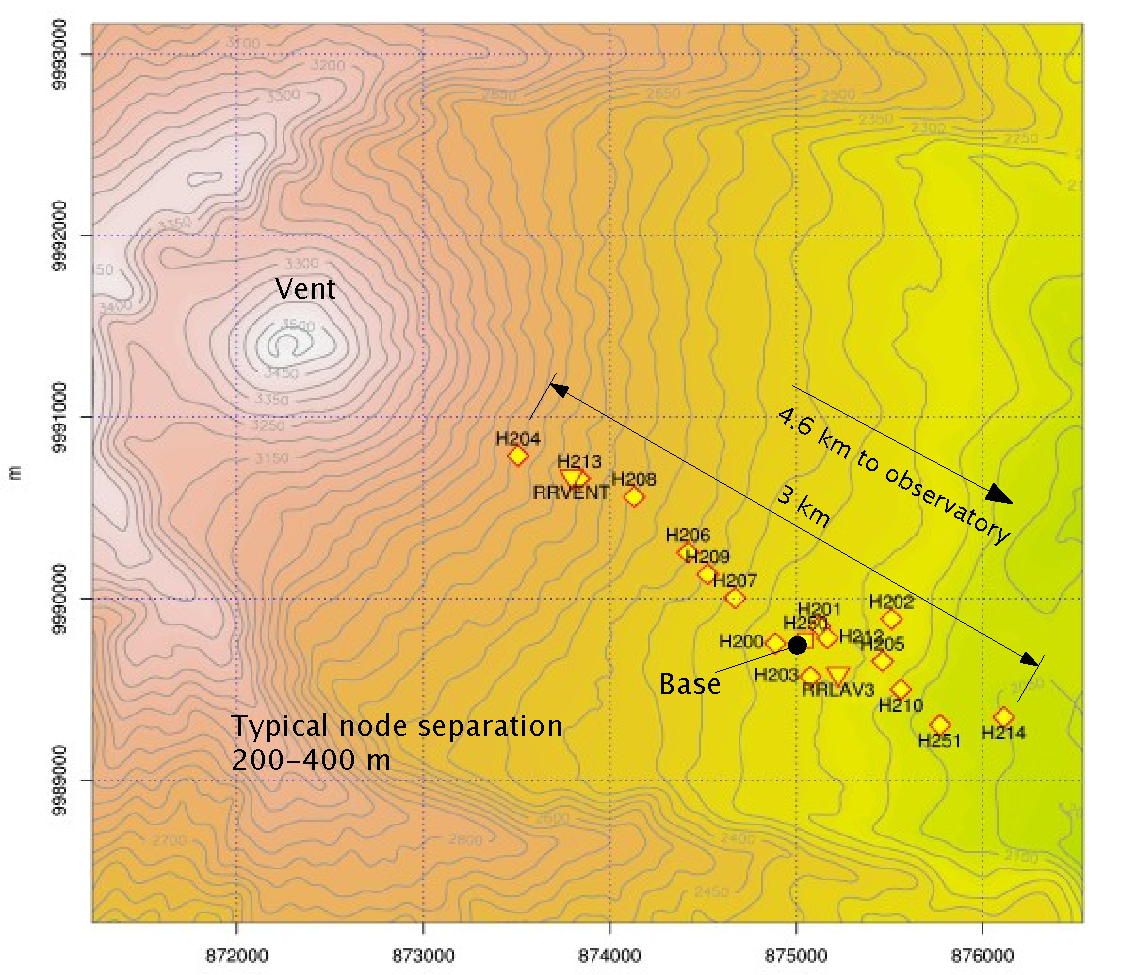
\includegraphics[width=0.8\hsize]{./5-evaluation/figs/pics/reventador-map.pdf}\\
\end{center}
\caption{\textbf{2005 deployment location.} The figure shows the location of
our second volcano deployment in 2005: 16 nodes deployed on Reventador
Volcano.}
\label{introduction-fig-deployment-map-2005}
\end{figure}

In total, we have performed three deployments of iterations of our system at
active volcanoes in Ecuador. Figs.~\ref{introduction-fig-deployment-map-2005}
and \ref{introduction-fig-deployment-map-2007} show the location and layout
of the second and third deployment. All three are summarized below:

\begin{figure}[t]
\begin{center}
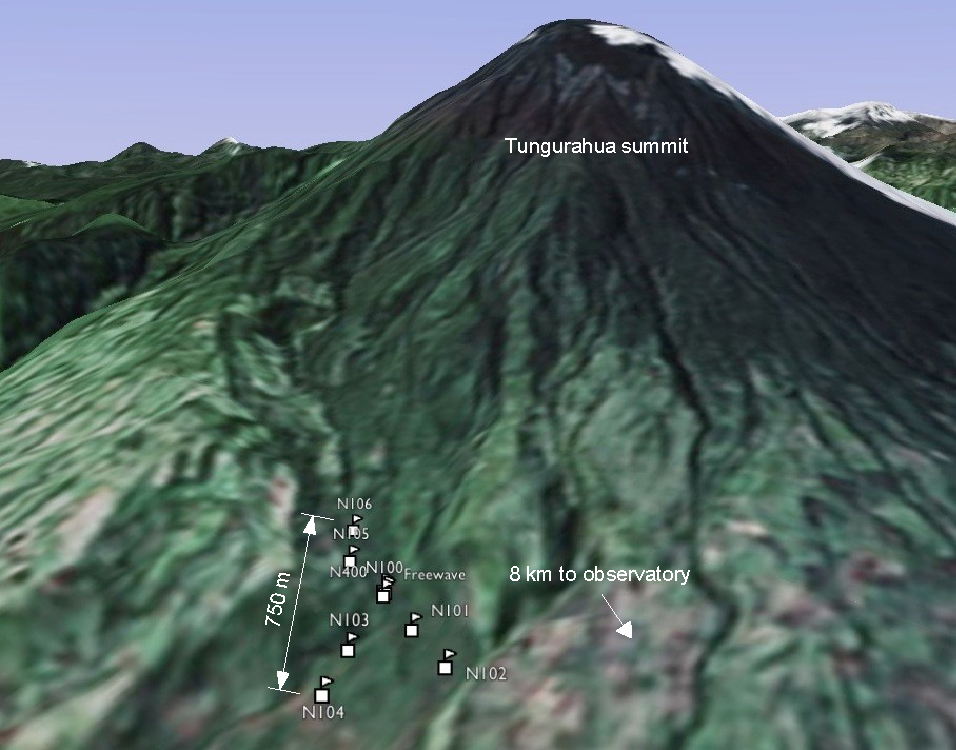
\includegraphics[width=0.8\hsize]{./6-lance/figs/deploy/deployment-map.pdf}\\
\end{center}
\caption{\textbf{2007 deployment location.} The figure shows the locations of
our third volcano deployment in 2007: eight nodes deployed on Tungurahua
Volcano.}
\label{introduction-fig-deployment-map-2007}
\end{figure}

\begin{enumerate}

\item \textbf{July, 2004, Tungurahua Volcano:} We deployed three infrasonic
monitoring nodes continuously transmitting at 102~Hz to a central aggregator
node, which relayed the data over a wireless link to the observatory
approximately 9~km away.  Our network was active from July 20--22, 2004, and
collected over 54~hours of infrasonic signals.

\item \textbf{August, 2005, Reventador Volcano:} This deployment featured a larger,
more capable network consisting of sixteen nodes fitted with seismoacoustic
sensors deployed in a 3~km linear array.  Collected data was routed over a
multi-hop network and over a long-distance radio link to a logging laptop
located at the observatory 9~km away from deployment site.  Over three weeks
the network captured 230 volcanic events.

\item \textbf{July, 2007, Tungurahua Volcano:} We returned to Tungurahua Volcano in
2007 and deployed eight sensor nodes in order to test Lance, a framework for
optimizing high-resolution signal collection. The network was operational for
a total of 71~hours, during which time we downloaded 77~MB of raw data.

\end{enumerate}

\section{Deploying on Volc\'{a}n Reventador}

Volc\'{a}n Reventador is located in northern Ecuador, a three hour drive from
the capital, Quito.  Long dormant, Reventador reawakened suddenly in 2002,
erupting with massive force.  Ash thrown into the air blanketed the streets
of Quito 100~km to the east, closing schools and the airport.  Pyroclastic
flows raced down the mountain flattening forests, displacing an oil pipeline,
and severing a major highway.  After 18 months of quiescence, renewed
activity began in November 2004.  During our deployment, Reventador's
activity was characterized by discrete, relatively small explosive events,
ejecting incandescent blocks, gas, and ash several times a day.
Corresponding seismic activity was manifested by explosion earthquakes,
extended-duration shaking (tremor), and shallow rock fracturing earthquakes
that may have been associated with magma migration within the volcano.

Several features of Volc\'{a}n Reventador made it ideal for our
experiment.  Reaching 3,500~meters at its peak, Reventador sits at a
low elevation compared to other Ecuadorean volcanoes making deployment
less strenuous.  Its climate is moderate with temperatures ranging
between 10 and 30 degrees Celsius.  Pyroclastic flows produced by the
large explosion in 2002 left large parts of the flanks denuded of
vegetation.  With the effectiveness of our radio antennas severely
degraded by obstacles to line-of-sight, the lack of vegetation
simplified sensor node positioning.

Our base while working at Reventador was the Hosteria El Reventador, a small
hotel located nearby on the highway from Quito to Lago Agria.  The hotel
provided us with space to set up our equipment and ran an electric generator
to power our laptops and other equipment at the makeshift observatory.

\subsection{Network Hardware}

Our network consisted of 16~stations equipped with seismic and acoustic
sensors.  Each station consisted of a Moteiv TMote Sky~\cite{moteiv} wireless
sensor network node, an 8~dBi~2.4GHz external omnidirectional antenna,
seismometer, microphone, and a custom hardware interface board.
Fourteen~nodes were fitted with a Geospace Industrial GS-11 geophone, a
single-axis seismometer with a corner frequency of 4.5~Hz, oriented in the
vertical plane of motion.  The remaining two~nodes were equipped with
triaxial Geospace Industries GS-1 seismometers with corner frequencies of
1~Hz, yielding separate signals in each of the three axes.

The TMote Sky is a descendant of the UC Berkeley Mica ``mote'' sensor node.
It features a Texas Instruments MSP430 microcontroller, 48~KB of program
memory, 10~KB of SRAM, 1~MByte of external flash memory and a 2.4GHz Chipcon
CC2420 IEEE 802.11.4 radio.  The TMote Sky was designed to run
TinyOS~\cite{tinyos-asplos00}, and all of our software development made use
of this environment.  We chose the TMote Sky for several reasons.  The MSP430
microprocessor provides a large number of configurable ports, easily
supporting external devices.  The large amount of flash memory was useful for
buffering collected data, as described below.

We built a custom hardware board to integrate the TMote Sky with the
seismoacoustic sensors.  The board features up to four Texas Instruments
AD7710 analog to digital converters (ADCs) providing up to 24~bits per
channel of resolution.  Although the MSP430 microcontroller provides on-board
ADCs, they are unsuitable for our application.  First, they provide only
16~bits of resolution while we required at least 20~bits.  Second,
seismoacoustic signals require an aggressive filter centered around 50~Hz.
Due to the infeasibility of implementing such a filter using analog
components, it is usually approximated digitally, requiring several factors
of oversampling.  To perform this filtering, the AD7710 is sampling at over
30~kHz while presenting an output word rate of 100~Hz.  The high sample rate
and computation required by digital filtering are best delegated to a
specialized device.

Each sensor node was powered by a pair of alkaline D~cell batteries.  The
remote location of our network made it important to choose batteries
maximizing node lifetime.  D~cells provided the best combination of low cost
and high capacity, and are able to power a node for over a week.
Approximately 75\% of the power drawn by each node is consumed by the sensor
interface board, primarily due to the high power consumption of the ADCs.
During our three week deployment we swapped batteries between 4~and~5 times.
This was more often than strictly necessary, but battery changes were often
performed while visiting nodes for other reasons.

\subsection{Sensor Network Device Enclosures and Physical Setup}

\begin{figure}[t]
\label{casestudy-fig-picture}
\begin{center}
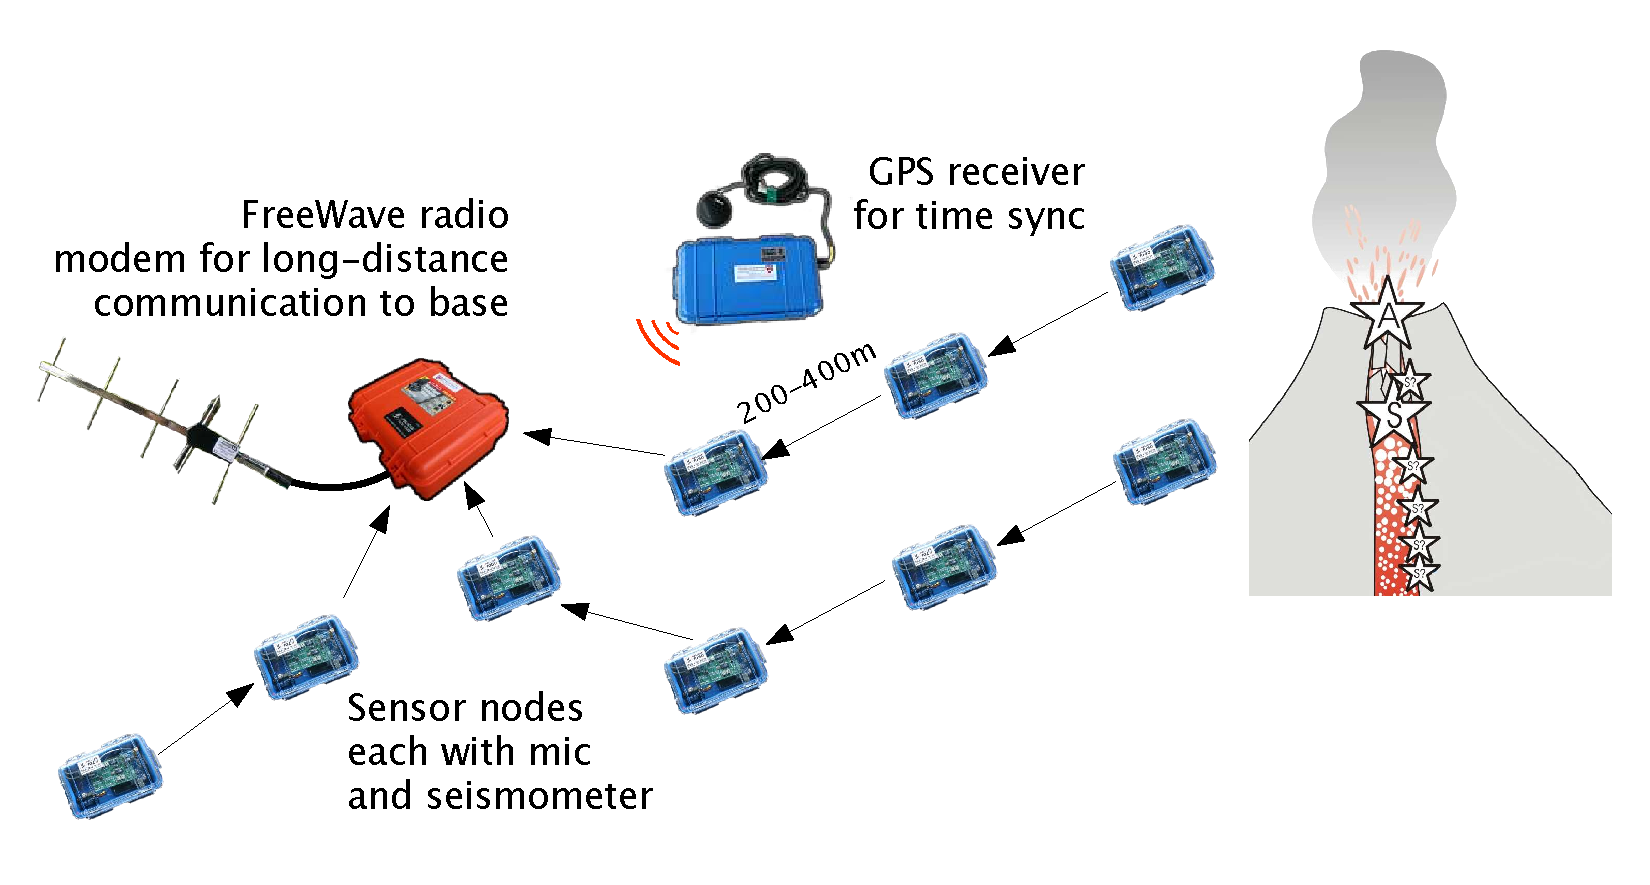
\includegraphics[width=0.7\hsize]{./4-casestudy/figs/schematic}
\end{center}
\caption{\textbf{Schematic representation of our sensor network
architecture.}}
\end{figure}

A single sensor network node, interface board, and battery holder were all
housed inside a small weatherproof and watertight Pelican case.  We installed
environmental connectors through the case allowing cables to external sensors
and antennae to be attached without opening the case and disturbing the
equipment inside.  When working in wet and gritty conditions these became a
tremendous asset.

\begin{figure}[t]
\begin{center}
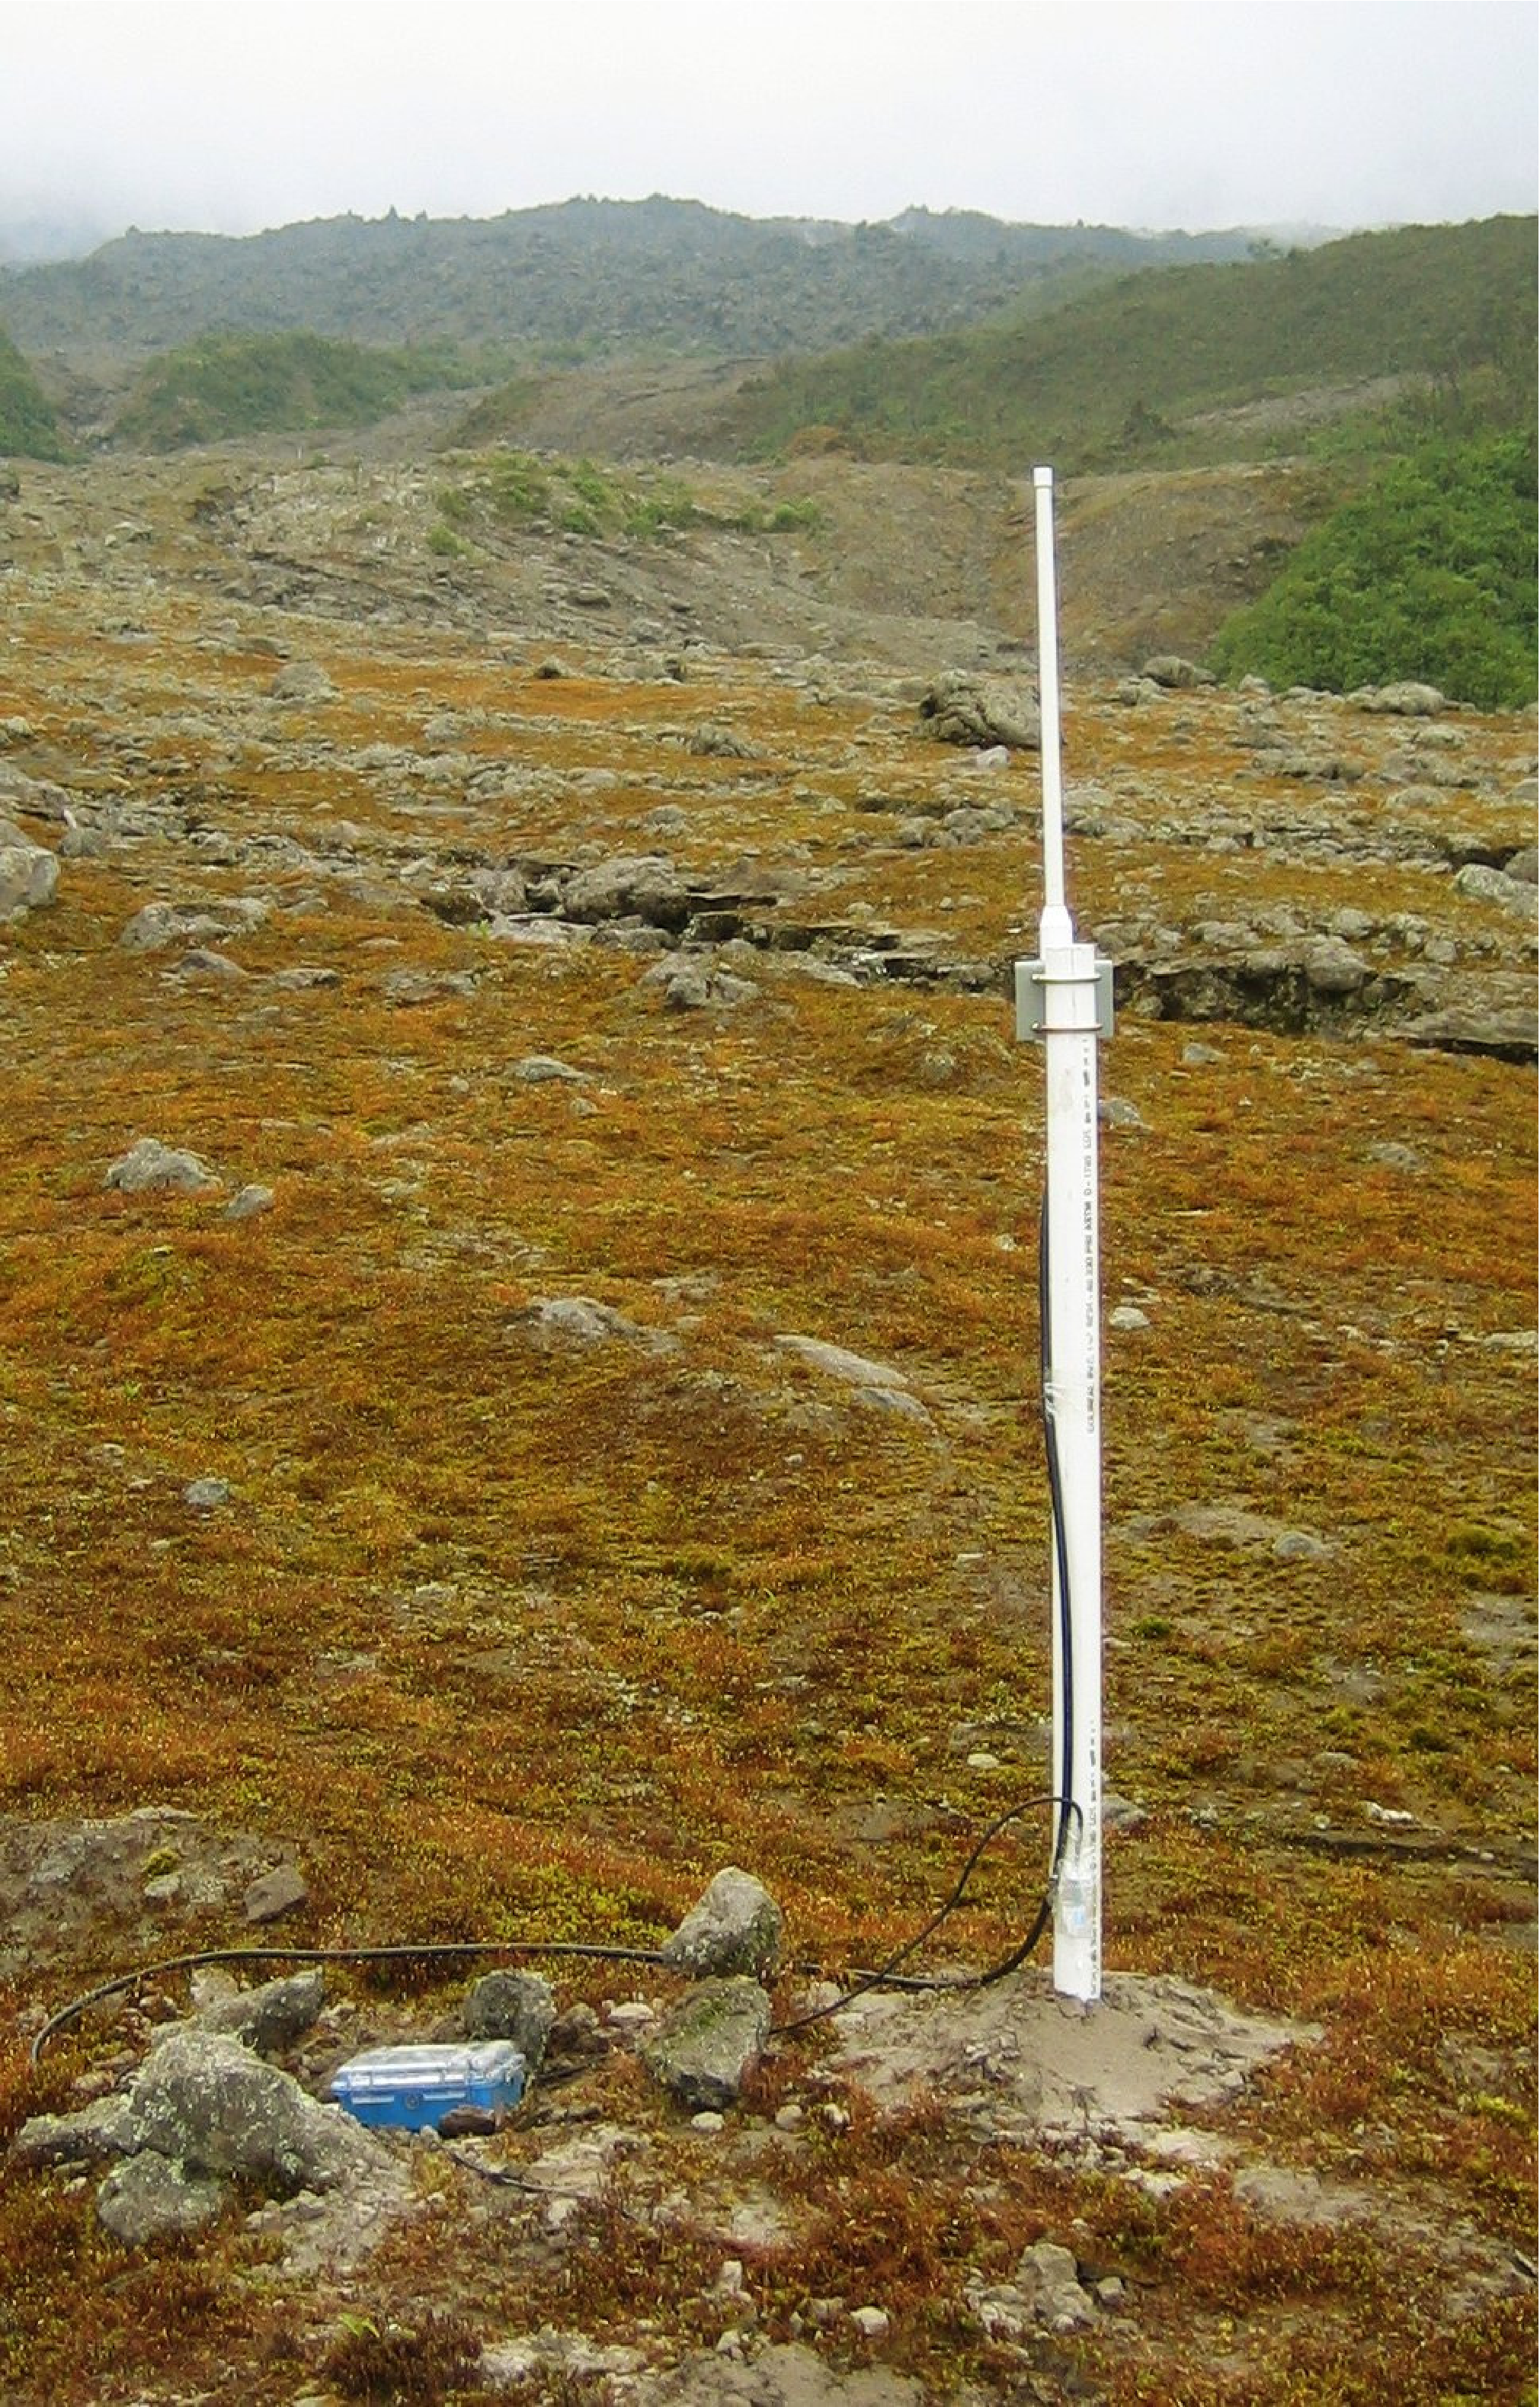
\includegraphics[width=0.7\hsize]{./4-casestudy/figs/Station}
\end{center}
\caption{\textbf{One of our two-component stations.  The blue Pelican
Case contains the wireless sensor network node and hardware interface board.
The external antenna is mounted on the PVC pole to reduce ground effects.
A microphone is taped to the PVC pole and a single seismometer is buried
nearby.}}
\label{fig-station}
\end{figure}

Installing a station involved covering the Pelican case with rocks to anchor
it and shield the contents from direct sunlight.  Cables were run from the
box to each sensor and to the antenna.  The antenna was elevated on a 1.5~m
length of PVC piping to reduce ground effects which reduce radio range.  The
seismometers were buried nearby, but far enough away to remain undisturbed by
any wind-induced shaking of the antenna pole.  The microphone was usually
mounted on the antenna pole and shielded from the wind and elements with
plastic tape.  Installation took a matter of minutes and the equipment was
sufficiently light and small that six stations could be carried in a large
pack.  The PVC poles were light but bulky and proved the most awkward part of
each station to cart around.

\subsection{Network Location and Topology}

We installed our stations in a roughly linear configuration, radiating away
from the vent and producing an aperture of over 3~km.  We attempted to
position the stations as far apart as the radios on each node would allow.
Although our antennas could maintain radio links of over 400~m, the geography
at the deployment site occasionally required installing additional stations
to maintain radio connectivity.  Other times we would deploy a node expecting
it to communicate with an immediate neighbor but later notice that that node
was bypassing its closest companion in favor of a node closer to the base
station.  Most nodes communicated with the base station over three or fewer
hops, but a few were moving data over as many as six.

In addition to the sensor nodes, several other pieces of equipment
were used.  Three Freewave~\cite{freewave} radio modems provided a
long-distance, reliable radio link between the sensor network and the
observatory laptop.  Freewave modems at the deployment site and the
observatory used a 9~dBi directional Yagi antenna to relay data via a
repeater station, installed on a hill with good line-of-sight to both
endpoints.  Each Freewave required a car battery for power, recharged
by solar panels.  A small number of Crossbow~\cite{xbow} MicaZ sensor
network nodes served in supporting roles.  One interfaced between the
network and the Freewave modem; another was attached to a GPS receiver
to provide a global timebase.

\begin{figure}[t]
\label{includegraphics-fig-plot}
\begin{center}
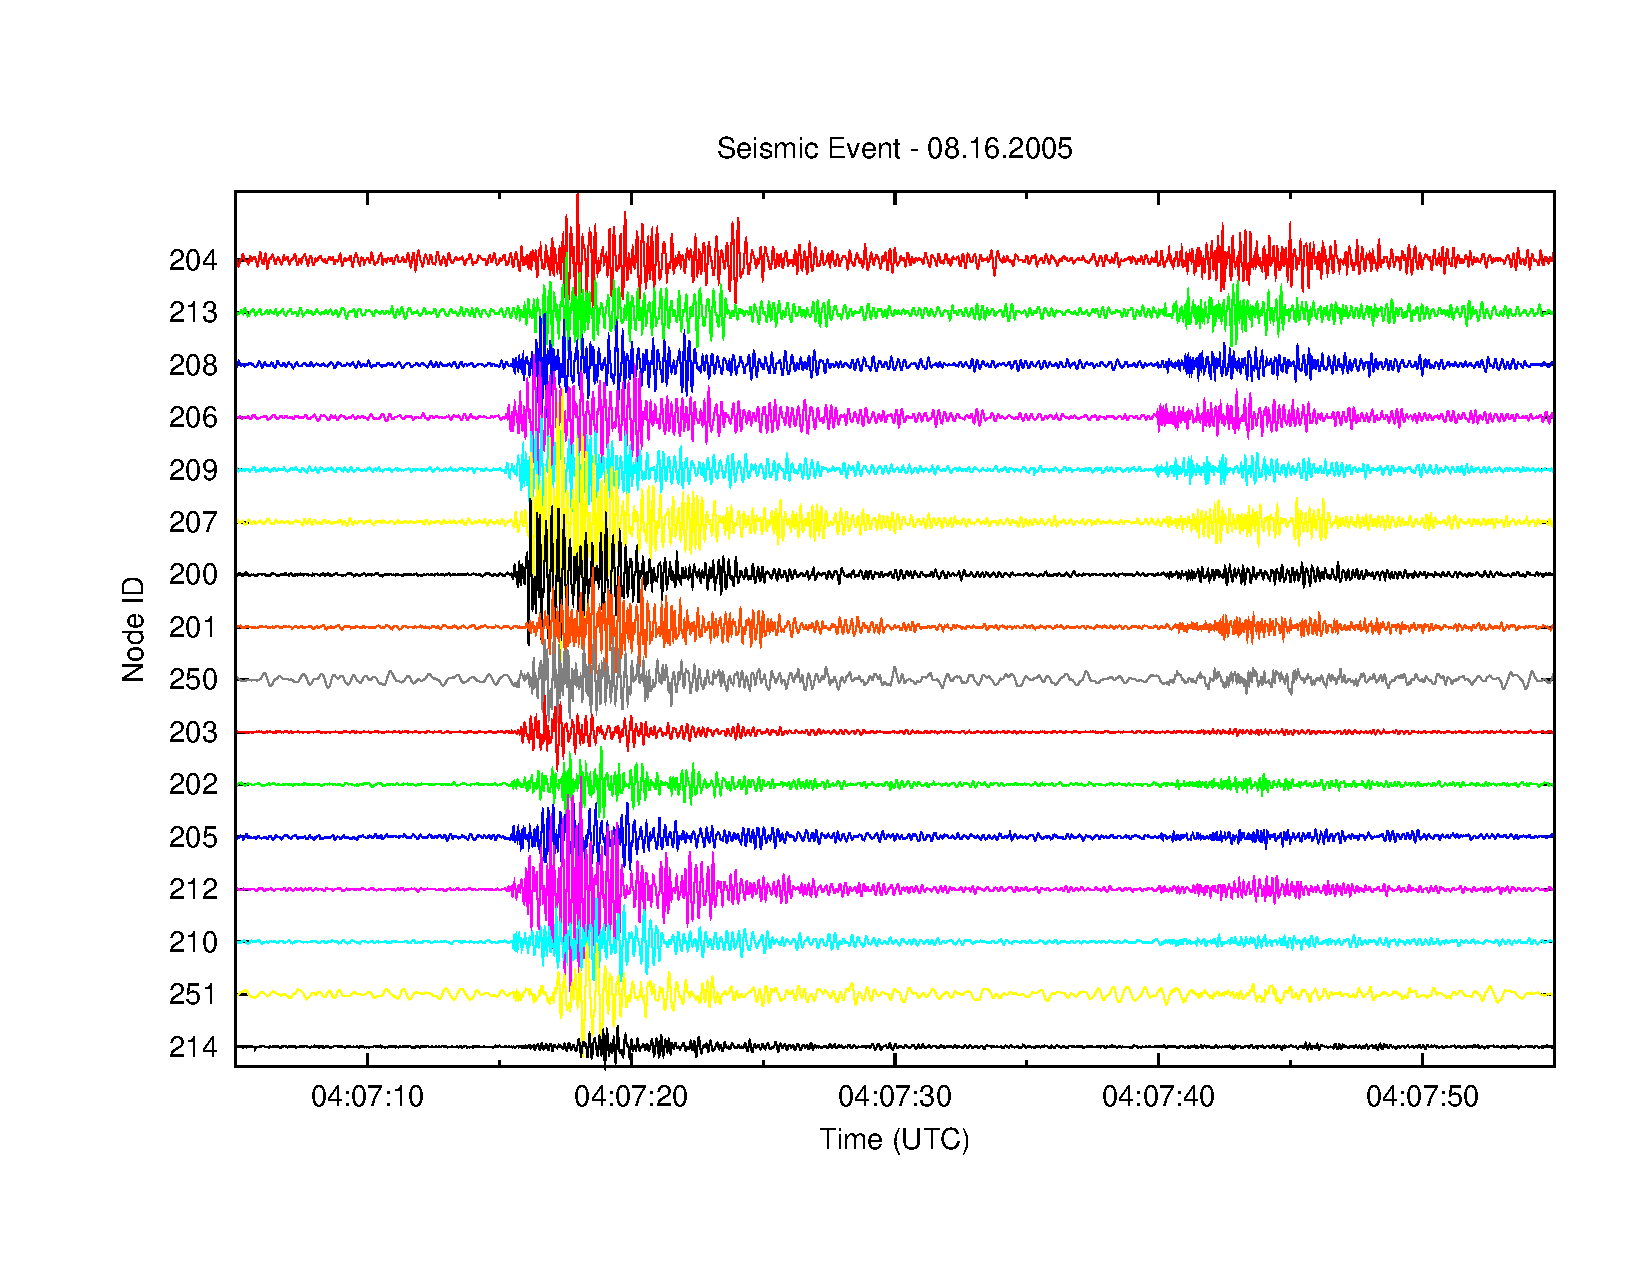
\includegraphics[width=0.7\hsize]{./4-casestudy/figs/TEST}
\end{center}
\caption{\textbf{Example of an event captured by our network.}  Only
seismic signals are shown.  The event shown was a Volcano Tectonic (VT) event
and had no interesting acoustic component.  Data shown has undergone several
rounds of post-processing including mapping to GMT time.}
\end{figure}

\begin{figure}[t]
\begin{center}
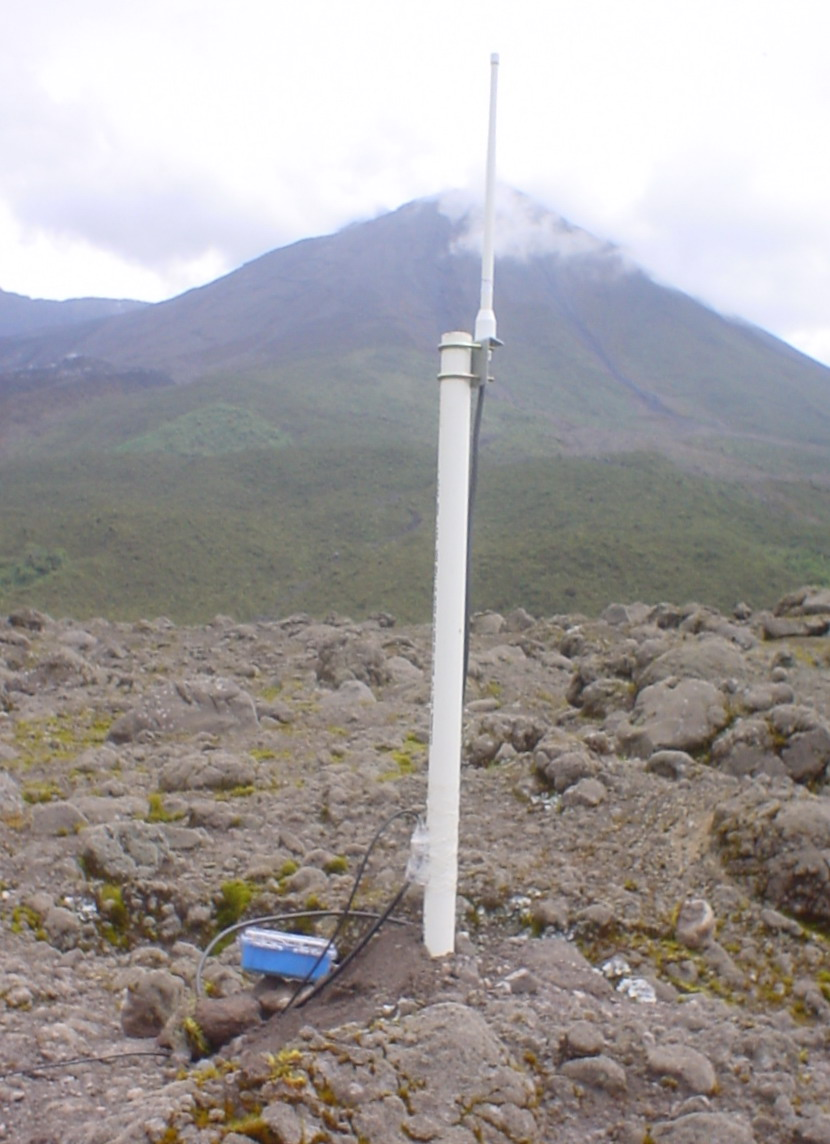
\includegraphics[width=0.7\hsize]{./4-casestudy/figs/Node-212-5}
\end{center}
\caption{\textbf{One of our two-component stations.} The blue Pelican
Case contains the wireless sensor network node and hardware interface board.
The external antenna is mounted on the PVC pole to reduce ground effects.
A microphone is taped to the PVC pole and a single seismometer is buried
nearby.}
\label{includegraphics-fig-station2}
\end{figure}


\section{Sensor Networks for Volcanic Monitoring}

Wireless sensor networks capable of assisting the study of volcanoes are exciting the
geophysics community.  The increased scale promised by lighter,
faster-to-deploy equipment will allow them to address scientific questions
beyond the practical reach of current equipment.  Today's
typical volcanic data collection station consists of a group of bulky,
heavy, power-hungry components, difficult to move and requiring car batteries
for power.  Remote deployments often require vehicle or helicopter assist to
install equipment and perform maintenance.  Local storage is also a
limiting factor.  Stations typically log data to a local Compact Flash card
which must be periodically retrieved, requiring researchers to regularly
return to each station.

These limitations make it difficult to deploy large networks of existing
equipment. Yet these large-scale experiments hold out the possibility of
achieving important insights into the inner workings of volcanoes.  For
example, volcanic tomography~\cite{lees-tomography} is the study of a
volcano's interior structure.  Collecting and analyzing signals from 
multiple stations can produce precise mappings of the internal structure of
the volcanic edifice.  In general the precision and accuracy of these
mappings increases as stations are added to the data collection network.
Studies such as these may help resolve debates over the physical processes at
work within the volcano's interior.

\subsection{Scientific Requirements}

The geophysics community has well-established tools and techniques used to
process the signals extracted by volcanic data collection networks.  These
analytical methods require that our wireless sensor network provide data of
extremely high fidelity.  A single missed or corrupted sample can invalidate
an entire record. Small differences in sampling rates between two nodes can
frustrate analysis.  Samples must be accurately time-stamped to allow
comparisons between nodes and between networks.

An important feature of volcanic signals is that much of the data analysis
focuses on discrete events, such as eruptions, earthquakes, or tremor
activity.  Although volcanoes differ significantly in the nature of their
activity, during our deployment many of the interesting signals at
Reventador spanned less than 60~sec and occurred at the rate of several dozen
per day. This allowed us to design the network to capture
time-limited events, rather than continuous signals. 

This is not to say that recording individual events is adequate to answer all
of the scientific questions volcanologists pose.  Indeed, understanding
long-term trends requires complete waveforms spanning long time intervals.
However, the low radio bandwidth of typical wireless sensor nodes makes them
inappropriate for these types of studies and for this reason we have focused
on triggered event collection.


Volcanic studies also require large inter-node separations to obtain
widely-separated views of the seismic and infrasonic signals as they
propagate.  Array configurations used often consist of one or more, possibly
intersecting, lines of sensors. The resulting topologies raise new challenges
for sensor network design, as much previous work has focused on dense
networks where each node has a large number of neighbors.  Linear
configurations also affect achievable network bandwidth, which degrades as
data must be transmitted over multiple hops.  Node failure poses a serious
problem in sparse networks because a single node failure can obscure a
large portion of the network.

\section{Sensor Network Application Design}
\label{sec-cs}

Given the current capabilities of wireless sensor network nodes, we set out to
design a data collection network meeting the scientific requirements outlined
above.  Before motivating our design we provide a high-level overview of
network operation.

\subsection{Typical Network Operation}

Each node samples two or four channels of seismoacoustic data at 100~Hz,
storing the data in local flash memory. Nodes also transmit periodic status
messages and perform time synchronization, as described below.
When a node detects an interesting event, it routes a message to the 
base station laptop.  
If enough nodes report an event within a short time interval, the laptop
initiates data collection which proceeds in a round-robin fashion. Between
30~and~60~seconds of data is downloaded from each node with a reliable data
collection protocol, ensuring that all buffered data from the event is
retrieved.  When data collection completes, nodes return to sampling 
and storing sensor data.

\subsection{Overcoming High Data Rates: Event Detection and Buffering}

% GWA : Changed numbers to KBS and fixed 50 Kbits/second number which is
% lowballing it.

When designing high data-rate sensing applications the most important
limitation of current sensor network nodes is low radio bandwidth.  IEEE
802.15.4 radios, such as the Chipcon CC2420, have raw data rates of around
30~KBytes/sec.  However overheads caused by packet framing, medium access
control (MAC), and multihop routing reduce the achievable data rate to less
than 10~KBytes/sec even in a single-hop network.

As a result, nodes can acquire data faster than they can transmit.  Simply
logging data to local storage for later retrieval is also infeasible for
these applications.  The TMote Sky has 1~MByte of flash memory which fills in
around 20 minutes on a two-component sensor node.  Fortunately, many
interesting volcanic events will fit in this buffer.  For a typical
earthquake or explosion at Reventador, 60~sec of data from each node is
adequate.  Therefore, we focused on developing a network to reliably collect
data for short, discrete events.  

% MDW: I don't think we need to use the term "local" event detector
% here. Also, you only need to italicize a term the first time it is
% used.
Sampled data is stored in the local flash memory of the node, which is
treated as a circular buffer. Each block of data is timestamped using
the local node time, which can later be mapped onto a global time,
as explained below. Each node runs an {\em event detector} on 
locally-sampled data. 
Good event detection algorithms produce high
event-detection rates while maintaining small false-positive rates.
The sensitivity of the detection algorithm links these two metrics: a more
sensitive detector correctly identifies more events at the
expense of producing more false positives.  

The data set produced by our previous deployment at Volc\'{a}n
Tungurahua~\cite{volcano-ewsn05} aided in the design of the event detector.
We implemented a short-term average/long-term average threshold detector,
which computes two exponentially-weighted moving averages (EWMAs) with
different gain constants. When the ratio between short-term average and the
long-term average exceeds a fixed threshold, the detector fires.  The
detector threshold allows nodes to distinguish between low-amplitude signals,
perhaps caused by distant earthquakes, and high-amplitude signals caused by
nearby volcanic activity.

When the event detector on a node fires it routes a small message to the base
station laptop.  If enough nodes report events within a certain time window
the laptop initiates data collection from the entire network (including nodes
that did not report the event). This global filtering prevents spurious event
detections from triggering a data collection cycle. Fetching 60~sec of data
from all 16 nodes in the network takes approximately one hour.  Because nodes
can only buffer 20 minutes of eruption data locally each node pauses sampling
and reporting events until its data has been uploaded.  As the latency
associated with data collection prevents our network from capturing all
events, optimizing the data collection process is a focus of future work.

%Buffering on each node is required because the identification and data
%retrieval takes time after which data from an event must remain available on
%the node.  We developed a component allowing us to treat the Flash memory as
%circular buffer.  Because our nodes filled this store in roughly 20 minutes
%and it typically took around one hour to download a single event from the
%entire network we disabled sampling on each node before beginning the global
%retrieval process.  

% GWA : Found a lot of this confusing and bordering on incorrect.  Cleaned up
% a bit.

\subsection{Reliable Data Transmission and Time Synchronization}

% Konrad: Rewrote this paragraph. I think it's clearer now.
Extracting high-fidelity data from a wireless sensor network is
challenging for two primary reasons.  First, the radio links are lossy
and frequently asymmetrical.  Second, the low-cost crystal oscillators
on these nodes have low tolerances and therefore the clock rates vary
across the network.  Much prior research has focused on addressing
these challenges.

%% Extracting high-fidelity data from a sensor network means coping with lossy
%% radio links and accurately time-stamping sampled data.  Radio links in
%% wireless sensor networks are lossy and frequently asymmetrical, and low-cost
%% crystal oscillators deployed on wireless sensor network nodes have low
%% tolerances and clock rates vary across the network.  Much prior research has
%% focused on addressing these challenges.

% MDW: I found the fetch description to be somewhat confusing; tried
% to reorganize.

We developed a reliable data-collection protocol, called {\tt Fetch}, that
retrieves buffered data from each node over a multihop network. Samples are
buffered locally in {\em blocks} of 256~bytes, tagged with a sequence number
and timestamp. During transmission each requested block is fragmented into a
number of {\em chunks}, each sent in a single radio message. The base station
laptop retrieves a block by flooding a request to the network using {\tt
Drip}, a variant of the TinyOS {\tt Trickle}~\cite{trickle}
data-dissemination protocol.  The request contains the target node ID, the
block sequence number, and a bitmap identifying missing chunks in the block. 

The target node replies by sending the requested chunks over a multihop path
to the base station.  The routing tree is constructed using {\tt
MultiHopLQI}, a variant of the TinyOS {\tt MintRoute}~\cite{awoo-multihop}
routing protocol modified to select routes based on the CC2420 Link Quality
Indicator (LQI) metric.  Link-layer acknowledgments and retransmissions are
used at each hop to improve reliability.  Retrieving one minute of stored
data from a two-channel sensor node requires fetching 206~blocks and can
takes several minutes to complete, depending on the quality of the multihop
path and the node's depth in the routing tree.

% MDW: I think we paint too rosy of a picture here: we need to explain that
% FTSP does not always work lest the reader think we relied on it blindly,
% and point to future work.
Scientific volcano studies require that sampled data be accurately
timestamped; in our case, a global clock accuracy of 1~msec was sufficient.
We chose to use the Flooding Time Synchronization Protocol (FTSP)~\cite{ftsp}
from Vanderbilt University to establish a global clock across our network.
The published accuracy of FTSP is very high and the TinyOS code was
straightforward to integrate into our application. One of the nodes used a
Garmin GPS receiver to map the FTSP global time to GMT.  Unfortunately, FTSP
occasionally exhibited unexpected behavior which prevented nodes from
accurately timestamping some data. We are currently developing techniques to
correct the timestamps of our data set based on the large amount of status
messages logged from each node, which provide a mapping from the local clock
to the FTSP global time.
% MDW: This is a nice setup for your next paper...

\subsection{Command and Control}

% MDW: This is not universally true!
A feature missing from most traditional volcanic data acquisition equipment
is real-time network control and monitoring. The long-distance radio link
between the observatory and the sensor network allowed the laptop to monitor
and control the network's activity. We developed a Java-based GUI for
monitoring the network's behavior and manually setting parameters, such as
sampling rates and event detection thresholds.  In addition, the GUI was
responsible for controlling data collection following a triggered event,
moving significant complexity out of the sensor network.  All packets
received by the laptop from the sensor network were logged, facilitating
later analysis of the network's operation.

The GUI also displayed a table summarizing network state, based on the
periodic status messages transmitted by each node.  Each table entry included
the node ID; local and global timestamps; various status flags; the amount of
locally-stored data; depth, parent, and radio link quality in the routing
tree; and the node's temperature and battery voltage.  This functionality
greatly aided sensor deployment, as a team member could rapidly determine
whether a new node had joined the network and the quality of its radio
connectivity.


\section{Conclusions}
\label{sec-conclusions}


%%%%%%%%%%%%%  THIS IS WHERE THE BIBLIOGRAPHY GOES %%%%%%%%%

\def\baselinestretch{0.92}
\begin{footnotesize}
\setlength{\itemsep}{2in}
\bibliographystyle{IEEEtran} \bibliography{IEEEComputing}
\end{footnotesize}
\end{document}
